\chapter{Number Representations}

\section{Dot notation}
\paragraph{} 
Extended Dot Notation
\begin{itemize}
	\item Posibit\quad  \(\newmoon\quad\in\quad \{\,\,0,\,\,\,1\}\) 
	\item Negabit\quad	\(\ocircle\quad\in\quad \{-1,0\}\)
	\item Twins
	\begin{enumerate}
		\item Unibit \quad \(\boxdot \quad\in\quad\{\,-1\,,\,1\}\)
		\item Doublebit \quad \(\blacksquare \quad\in\quad\{\,0,\,2\}\)
			\item NegaDoublebit\quad\(\square\quad \in\quad\{\,-2,0\}\)  
	\end{enumerate}

\end{itemize}

Some BSD representation using Extended Dot Notation
\begin{itemize}
	\item \textit{(n,p)} encoding \begin{align*}
		\ocircle\ocircle\ocircle\ocircle\ocircle\\
		\newmoon\,\,\newmoon\,\,\newmoon\,\newmoon\,\newmoon
	\end{align*}
	\item \textit{2's-compl, encoding}
	\begin{align*}
		\square\,\square\,\square\,\square\,\square\\
		\newmoon\,\newmoon\,\newmoon\,\newmoon\,\newmoon
	\end{align*}
	\item  \textit{2's-compl, encoding}
	\begin{align*}
		\ocircle\ocircle\ocircle\ocircle\ocircle\quad\\
		\newmoon\,\,\newmoon\,\,\newmoon\,\newmoon\,\newmoon
	\end{align*}
\end{itemize}
\paragraph{}
Unsigned positive-radix number: \begin{align*}
		\newmoon\,\newmoon\,\newmoon\,\newmoon\,\newmoon\,\newmoon\,\newmoon\,\newmoon
\end{align*}
\textit{2's Complement number}:\begin{align*}
		\ocircle\,\newmoon\,\newmoon\,\newmoon\,\newmoon\,\newmoon\,\newmoon\,\newmoon
\end{align*}
Negative-Radix number:\begin{align*}
		\ocircle\,\newmoon\,\ocircle\,\newmoon\,\ocircle\,\newmoon\,\ocircle\newmoon\,\quad
\end{align*}
Multiplication for signed numbers:
\begin{align*}
	\ocircle\quad\newmoon\quad\newmoon\quad\newmoon \\
	\mathcal{\times}\,\,\ocircle\,\,\,\,\newmoon\quad\newmoon\quad\newmoon\\
	\hline\\
	\ocircle\quad\newmoon\quad\newmoon\quad\newmoon\\
	\ocircle\quad\newmoon\quad\newmoon\quad\newmoon\quad\,\,\,\,\\
	\ocircle\quad\newmoon\quad\newmoon\quad\newmoon\qquad\quad\,\,\\
	\newmoon\quad\ocircle\quad\ocircle\quad\ocircle\quad\qquad\qquad\\
	\hline\\
	\ocircle\quad\newmoon\quad\newmoon\quad\newmoon\quad\newmoon\quad\newmoon\quad\newmoon\quad\newmoon
\end{align*}\\

Addition for unsigned positive-radix numbers:
\begin{align*}
	\ocircle\quad\newmoon\quad\newmoon\quad\newmoon \,\\
	\textbf{+}\quad\ocircle\quad\newmoon\quad\newmoon\quad\newmoon\\
	\hline
	\quad\ocircle\quad\newmoon\quad\newmoon\quad\newmoon\,\,\,\,\,\newmoon
\end{align*}\\
Multiplication for unsigned positive-radix numbers:
\begin{align*}
	\newmoon\quad\newmoon\quad\newmoon \\
	\mathcal{\times}\quad\newmoon\quad\newmoon\quad\newmoon\\
	\hline\\
	\newmoon\quad\newmoon\quad\newmoon\quad\newmoon\\
	\newmoon\quad\newmoon\quad\newmoon\quad\newmoon\quad\quad\\
	\newmoon\quad\newmoon\quad\newmoon\quad\newmoon\qquad\qquad\\
	\newmoon\quad\newmoon\quad\newmoon\quad\newmoon\qquad\qquad\qquad\\
	\hline\\
	\newmoon\quad\newmoon\quad\newmoon\quad\newmoon\quad\newmoon\quad\newmoon\quad\newmoon\quad\newmoon
\end{align*}\\
Addition for unsigned positive-radix numbers:
\begin{align*}
	\newmoon\quad\newmoon\quad\newmoon \\
	\textbf{+}\quad\newmoon\quad\newmoon\quad\newmoon\\
	\hline\\
	\quad\newmoon\quad\newmoon\quad\newmoon\quad\newmoon
\end{align*}\\
\\
There are many other number representations but the most important ones are:
\begin{enumerate}
	\item \textbf{2's} Complement
	\item \textbf{Binary Stored-carry} or \textbf{Carry-saved} format
	\item \textbf{Binary floating point number } (IEEE 754)
	\item \textbf{BCD}
\end{enumerate}

\section{Signed Number Representations}
\subsection{Signed-Magnitude Representation}
Definition: The \textbf{most left bit} is the \textbf{sign bit} (s) \[
	\mathbf{if}
\left\{\begin{array}{cl}
	s\,=\,0 & \Longrightarrow \text{positive number}\\s\,=1 & \Longrightarrow \text{negative number} 
\end{array}\right\}
\]
Numbers of this Representation type are \textit{fix-point and with no fraction}\\
In \textit{Radix r} the number \(k\)  of digits needed for representing [0,max] is
\[
	k\,=\,\left\lfloor\,log_{r}max\,+\,1 \right\rfloor\,+1\,=\,\left\lceil log_{r}(max+1) \right\rceil 
\]
\\
Example: for Radix=2 and range is [0,7] how many digits are needed?
\\\\Solution: \(k\,=\left\lceil log_{2}(7+1) \right\rceil \Longrightarrow\, 3\) so there are 3 digits are needed for representing this digit set\\\\
\textbf{Disadvantages of Signed-Magnitude Representation}
\begin{enumerate}
	\item Because of Symmetric nature of this representation there will be two \(0\)s with different signs \(\pm0\). This is unavoidable in Radix-2 Symmetric Systems.
	\item More overhead and thus more delay because of \(\pm0\) existence.
\end{enumerate}
Finally the Digit set of \textbf{Signed-Magnitude Representation} is 
\[
	\big[-(2^{k-1}\,-\,1)\,,2^{k\,-\,1}\,-1\big]
\]
\begin{figure*}
	\centering
	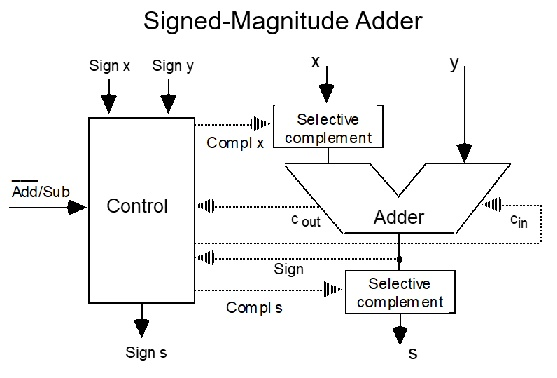
\includegraphics{smadder.jpg}
	\caption[short]{Adding signed-magnitude numbers using precomplementation and postcomplementation.}
\end{figure*}

\subsection{Biased Representations}
\paragraph{}
As the name suggests\textit{\textbf{ a bias}} is applied to the \textbf{signed number}; which then can be used for conversion from\textbf{ Signed} to \textbf{Unsigned} numbers.\\
The\textbf{ Digit set }can be shown as \( \mathbf{{[-bias,max-bias}]} \); using values from \textbf{0} to \textbf{max}, this is often called \textbf{"excess-bias"}. Most notable examples are \textbf{"excess-3" or (BCD)} and \textbf{"excess-128"} (is used for simpler hardware) coding.
\paragraph{}
\textbf{Arithmetic with Biased Numbers}
\begin{align*}
	x+y-bias=(x+bias)+(y+bias)-bias \\
	x-y+bias=(x+bias)-(y+bias)+bias\\
	\text{A power of 2 bias }\mathbf{2^{k-1}}\text{simplifies the addition and Subtraction}
\end{align*}
Comparison of biased numbers:\\
The process is the same as  ordinary unsigned numbers.

\subsection{Complement Representations}
Arithmetic with Complement Representations:\\\\
\begin{table}[h]
	\centering
	\resizebox{\columnwidth}{!}{
\begin{tabular}{|c||c||c||c|}
	\hline
	\rule[-1ex]{0pt}{2ex} Operation & Computer to be performed by mod M & Correct result with no overflow & Overflow Condition \\
	\hline
	\rule{0pt}{1ex} (+x)+(+y) & x+y & x+y & x+y > P \\
	\hline
	\rule{0pt}{2ex} (+x) + (-y) & x + (M - y)  & x - y if  y= x , M -(y- x) if  y $>$ x
	& None \\
	\hline
	\rule{0pt}{2ex} (-x) + (+y) & (M-x)+y & y - x if x = y, M - (x - y) if x $>$ y
	& None \\
	\hline
	\rule{0pt}{2ex} (-x) + (-y) & (M - x) + (M - y) & M -(x + y) & x + y $>$ N
	\\
	\hline

\end{tabular}
}
\end{table}
\subsubsection{2's Complement (Radix-Complement)}
2's-complement system for r = 2\\
\( M = 2^{k} \)\\
\( 2^{k} – x = [(2^{k} – ulp) – x] + ulp       \)    
\( \Rightarrow x^{compl }+ ulp \)

Range of representable numbers in with k whole bits:
from \[–2^{k–1} \to  2^{k–1} – ulp\]
for number $x \Longrightarrow $ \(2^{k}-x\quad=\,\,\,[(2^{k}-ulp)-x]+ulp\quad=x^{compl}+ulp\)    
\textit{adding ulp is a slow process because in the worse case it involves full carry propagation}\\
this ulp addition usually can be avoided.
\subsubsection{1's Complement (Digit Complement)}
1's-complement system for r = 2\\
\(M = 2^{k} – ulp \)\\
\((2^{k} – ulp) – x = x^{compl'} \)\\
Range of representable numbers in with k whole bits:

from \[–2^{k–1} + ulp \to 2^{k–1} – ulp \]
\emph{In terms of hardware, the carry-out of a (k+1) bit adder should be directly connected to its carry-in;  which is  know as end-around carry }
\subsubsection{Radix-Complement Versus Digit-Complement Comparison }
\begin{table}[h]
	\centering
	\resizebox{\columnwidth}{!}{
	\begin{tabular}[t]{|c|c|c|}
			\hline 	
			\rule[-1ex]{0pt}{2ex} Feature/Property & Radix Complement &  Digit Complement \\
			\hline
			\rule[-1ex]{0pt}{2ex} Symmetry(\(P=N\))? & Possible for odd r (Radices of practical interest are even) & Possible for even r \\
			\hline
				\rule[-1ex]{0pt}{2ex} Unique zero? & Yes  & No\\
			\hline
			\rule[-1ex]{0pt}{2ex}Complementation  & Complement all digits and add ulp & Complement all digits  \\
			\hline
			\rule[-1ex]{0pt}{2ex}Mod-M addition  &Drop the carry-out& End-around carry  \\
			\hline
	\end{tabular}
}
\end{table}
The following implementation mitigates \textit{Complementation } for Radix Complement, thus making it the most favored choice in all modern systems
\begin{figure*}[ht]
		\centering
	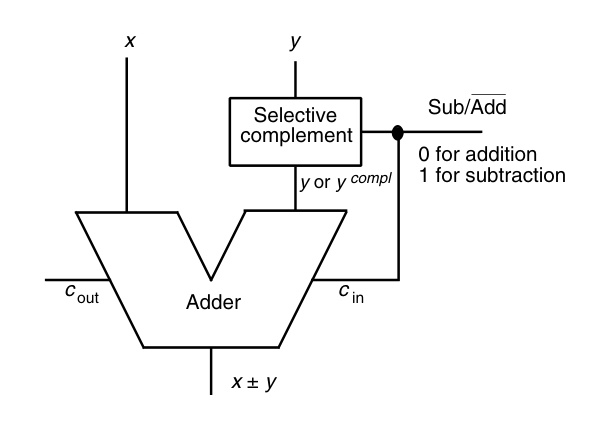
\includegraphics{2scompl.jpg}
	\caption[short]{Adder/subtractor architecture for 2's-complement numbers..}
\end{figure*}

\subsubsection{Sign Extended 2's and 1's Complements}
\paragraph{}
When there is a need for extending a number to fit the size of the operation the following procedure must be followed based on the Complement representation type\\
The general form of a number is depicted as follow:
\[
	x_{k-1}x_{k-2}\cdots\,x_{1}x_{0}.x_{-1}x_{-2}\cdots\,x_{-l}
\]
\emph{Sign Extended 2's-Complement}:\\
Algorithm for 2's-Complement sign extension
\begin{enumerate}
	\item Extend the left side by replication of the \textbf{sign bit} \(x_{k-1}\) from the left :
	\[
			\cdots 	x_{k-1} 	x_{k-1} 	x_{k-1} 	x_{k-1}x_{k-2} \cdots\,x_{1}x_{0}.x_{-1}x_{-2}\cdots\,x_{-l}
	\]
	\item And  extend the right side by padding zeros:
	\[
			\cdots 	x_{k-1} 	x_{k-1} 	x_{k-1} 	x_{k-1}x_{k-2} \cdots\,x_{1}x_{0}.x_{-1}x_{-2}\cdots\,x_{-l},0,0,0,0\cdots
	\] 
\end{enumerate}
\emph{Sign Extended 1's-Complement}:\\
Algorithm for 1's-Complement sign extension:
The number must be \textbf{sign extended from both sides}
\[
	\cdots 	x_{k-1} 	x_{k-1} 	x_{k-1} 	x_{k-1}x_{k-2} \cdots\,x_{1}x_{0}.x_{-1}x_{-2}\cdots\,x_{-l}x_{k-1} x_{k-1} x_{k-1} x_{k-1} \cdots
\]
\section{Direct and Indirect Signed Arithmetic}
